\begin{figure}[t!]
  \centering
  \begin{subfigure}[t]{0.65\textwidth}
    \centering
    \begin{tikzpicture}[xscale=0.7,yscale=0.6]
      \footnotesize
      % variables
      \draw ( 2, 0) node(Xt){$\fsmState{t}$} ;
      \draw (10.5, 0) node(Xtplus){$\fsmState{t+1}$} ;
      \draw (7.5, 1.5) node(Kt){$K_{t+1}$} ;
      \draw (4.5, 1.5) node(St){$S_t$};
      % operations
      \draw (2.5, 1) rectangle (3.5, 2) node[pos=0.5]{$\filter$} ;
      \draw ( 4, -0.5) rectangle (5, 0.5) node[pos=0.5]{$\shiftR$} ;
      \draw ( 6, -0.5) rectangle (7, 0.5) node[pos=0.5]{$\mixC$} ;
      \draw ( 7.5, 0) node(add)[inner sep=0pt]{$\boxplus$} ;
      \draw (8, -0.5) rectangle (9, 0.5) node[pos=0.5]{$\subW$} ;
      % arrows
      \draw[->] (Xt) -- (4, 0) ;
      \draw[->] (3, 0) -- (3, 1) ;
      \draw[->] (3.5, 1.5) -- (St) ;
      \draw[->] (5, 0) -- (6, 0) ;
      \draw[->] (7, 0) -- (add) ;
      \draw[->] (Kt) -- (add) ;
      \draw[->] (add) -- (8, 0) ;
      \draw[->] (9, 0) -- (Xtplus) ;
    \end{tikzpicture}
    \caption{\label{fig:notations}Notation throughout clocks.}
  \end{subfigure}
  \hfill
  \begin{subfigure}[t]{0.34\textwidth}
    \centering
    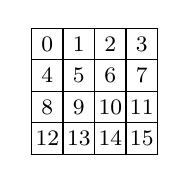
\begin{tikzpicture}[xscale=0.4,yscale=0.4]
      \footnotesize
      \foreach \i in {0,1,2,3}{
        \foreach \j in {0,1,2,3}{
          \draw (\i,\j) rectangle (\i+1,\j+1) ;
        }
      }
      \draw (.5,3.5) node {$0$};
      \draw (1.5,3.5) node {$1$};
      \draw (2.5,3.5) node {$2$};
      \draw (3.5,3.5) node {$3$};

      \draw (.5,2.5) node {$4$};
      \draw (1.5,2.5) node {$5$};
      \draw (2.5,2.5) node {$6$};
      \draw (3.5,2.5) node {$7$};

      \draw (.5,1.5) node {$8$};
      \draw (1.5,1.5) node {$9$};
      \draw (2.5,1.5) node {$10$};
      \draw (3.5,1.5) node {$11$};

      \draw (.5,.5) node {$12$};
      \draw (1.5,.5) node {$13$};
      \draw (2.5,.5) node {$14$};
      \draw (3.5,.5) node {$15$};
    \end{tikzpicture}
    \caption{\label{fig:numbering}Numbering in the FSM.}
  \end{subfigure}
  \hfill~
  
  \caption{\label{fig:notations-all}Our notations. Note that the numbering of the digits differs from the one traditionally used for the AES.}
\end{figure}


% Leo: ce qui suit est pour qu'emacs compile bien l'article, pas touche !
%%% Local Variables:
%%% mode: latex
%%% ispell-local-dictionary: "english"
%%% TeX-master: "../main"
%%% End:



